\section{Beispiel Kapitel Nummer 1}
In den folgenden Beispielkapiteln werden die wichtigsten Features von \LaTeX\:demonstriert. Diese sollen den Einstieg in das Programm Overleaf und die generelle Umgebung erleichtern. Diese Datei soll ein Grundgerüst für zukünftige Abschlussarbeiten sowie Praktikumsberichte und ähnliches darstellen. Es ist erwünscht, dass der Inhalt des Dokuments gelöscht wird, um die Formatierung zu verwenden.\\
Der folgende Text ist als Code in Kombination mit der kompilierten PDF zu lesen.\\

\subsection{Grundlagen}
Die wichtigsten Grundlagen findet man in sogenannten Cheatsheets, in welchen auf wenigen Seiten die wichtigsten Befehle von \LaTeX\:zusammengefasst sind. Ein solches Cheatsheet findet man unter:\\ \url{https://wch.github.io/latexsheet/} \\Beim Auseinandersetzen mit \LaTeX\: werden die wichtigsten Befehle schnell zu Automatismen, was die Benutzung erleichtert.\\
Im Folgenden werden die wichtigsten Grundlagen zum Einfügen von Tabellen, Grafiken und Zitationen kurz dargestellt. Auch Mathematische und Chemische Gleichungen lassen sich problemlos in \LaTeX einfügen, jedoch wird darauf nicht näher im Folgenden eingegangen, da das Vorgehen unter "Math mode" im verlinkten Cheatsheet beschrieben ist.

\pagebreak

\subsubsection{Tabellen}
Für Tabellen gibt es online verschiedene "LATEX Tabellengeneratoren", zum Beispiel:\\
\url{https://www.tablesgenerator.com/#}\\
Tabellen sehen dann wie folgt aus:

\begin{table}[H]
\begin{tabular}{|l|l|l|}
\hline
Beispiel & Test 1 & Test 2        \\ \hline
Farbe    & Grün   & Ultra-Violett \\ \hline
\end{tabular}
\caption[Beispiel Tabelle]{Beispiel Tabelle}
	\label{Tabelle 1}
\end{table}

Die Position der Tabelle (genauso Grafiken) wird über die eckigen Klammern hinter \textbackslash begin gesteuert.\\ Sowohl bei Abbildungen als auch bei Tabellen fügt man eine \textbackslash caption und ein \textbackslash label ein. Die Caption ist für das Tabellen- und Abbildungsverzeichnis, wohingegen das Label für die Referenzierung im Text ist (Beispiel: Tabelle \ref{Tabelle 1}). Falls man nun weitere Tabellen hinzufügt wird an dieser Stelle immer die entsprechende Nummer der Beispiel Tabelle auftauchen.
\pagebreak


\subsubsection{Grafiken}
Grafiken werden direkt in Overleaf hochgeladen. Man kann dann verschiedene Ordner (Oben Links) anlegen, um die Grafiken in sich zu strukturieren.

\begin{figure}[H]
 \centering
 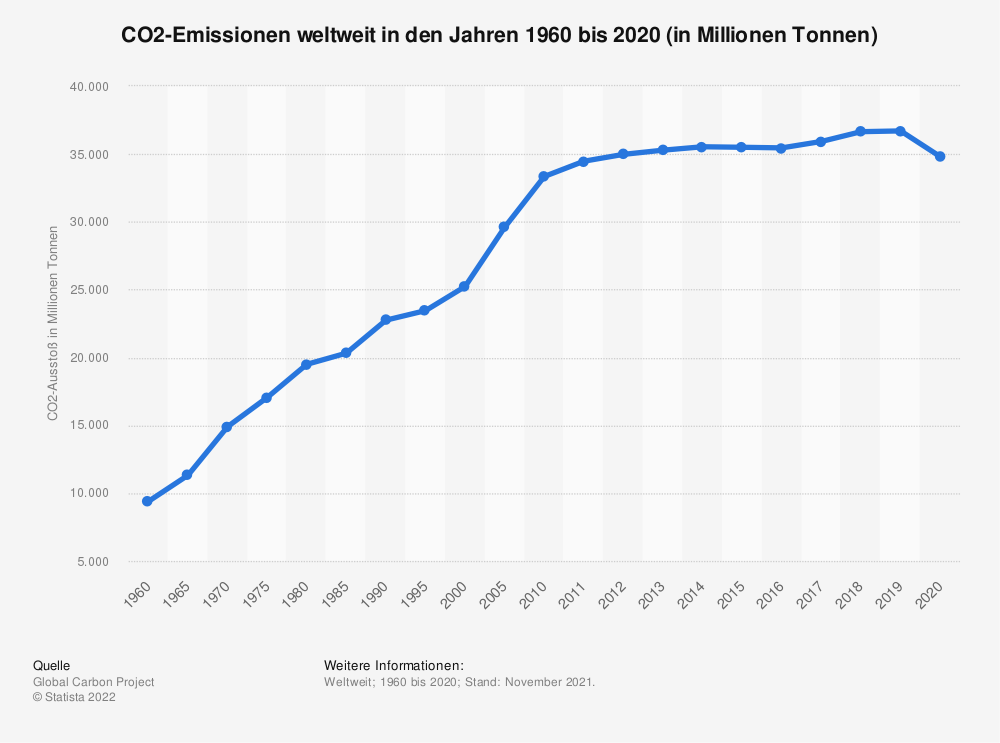
\includegraphics[width=0.8\textwidth]{Bilder/Beispiel Bilder/Klimawandel.png}
 \caption{Erschreckende Statistik zum Klimawandel}
 \label{Klimawandel}
\end{figure}
Auch hier kann  die Abbildung referenziert werden. So zeigt Abbildung \ref{Klimawandel} den weltweiten Kohlenstoffdioxid Ausstoß in Tonnen im Zeitraum von 1960 bis 2020. Die Abbildung wird auch automatisch im Abbildungsverzeichnis aufgeführt. In den eckigen Klammern können die Maße der Abbildung geändert werden.
\pagebreak
\subsubsection{Zitationen und Bibliografie}
Für die Zitationen werden in einem gesonderten Dokument alle Quellen hinterlegt. Dieses Dokument heißt hier "Referenzen.bib". In diesem Dokument können alle Arten von Quellen hinterlegt werden. Viele wissenschaftlichen Websiten bieten BIBTEX Zitationen an. Besonders hilfreich sind Literatur Generatoren wie:\\
\url{https://www.literatur-generator.de},\\
welche Zitationen zu Büchern und Artikeln für den Benutzer erzeugen können.\\
Zitationen sehen dann im Text wie folgt aus: \cite{Gates2021}. Das Aussehen der Zitationen kann bei dem benutzten Package geändert werden. Des Weiteren erstellt \LaTeX ein automatisiertes Literaturverzeichnis mit den benutzten Quellen.